% \section{Results}

We presented $\Rnum$ as the product of the classical reproduction number, $\beta/\gamma$, and the proportional reduction due to testing and isolation, $1-\Delta$, \eqref{R0}.
We can use the formula for $\Delta$ \eqref{eq:del4a} to make a number of straightforward inferences about parameters that affect $\Rnum$ monotonically, i.e., for which the associated partial derivative of $\Delta$ always has the same sign (see Appendices).

\begin{enumerate}

\item \label{p1:eta} Increasing isolation efficacy for waiting ($\theta\_w$) and confirmed-positive ($\theta\_c$) individuals always increases $\Delta$ (Eqs.~\ref{eq:del4_theta},~\ref{eq:d_del4_thetac},~\ref{eq:d_del4_thetaw});
\item \label{p1:rho} Higher testing intensity $\rho$ increases $\Delta$ if
%% \begin{enumerate} \item
testing is random (all $w_X$ equal) or testing intensity ($\rho$) is small (Eq.~\ref{eq:dd3dr}).
%% \end{enumerate}
\item \label{p1:omega} Increasing the rate of test return ($\omega$) always increases $\Delta$ if waiting individuals do not isolate ($\theta\_w=0$) (Eq.~\ref{eq:dlindo}).
\item \label{p1:w} Increasing testing focus, i.e., changing the testing weights from random ($w_S=w_I$) toward targeted  ($w_S<w_I$), always increases $\Delta$ (Eq.~\ref{eq:d_del_wis}).
\end{enumerate}

\newpage
\begin{figure}[h!]
\centering
\begin{subfigure}[t]{.49\textwidth}
\centering
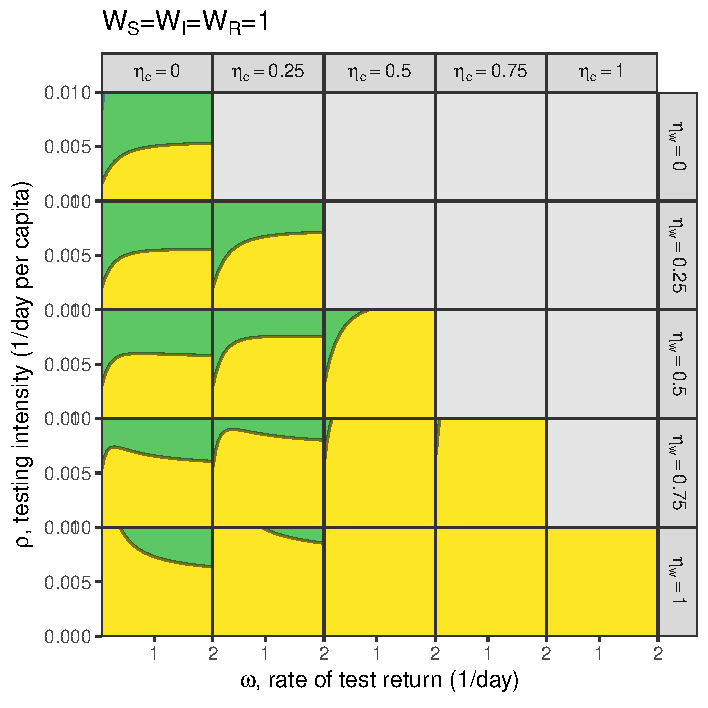
\includegraphics[width=\linewidth]{codes/R0contour_random.pdf}
\caption{}\label{p.a}
\end{subfigure}
%
\begin{subfigure}[t]{.49\textwidth}
\centering
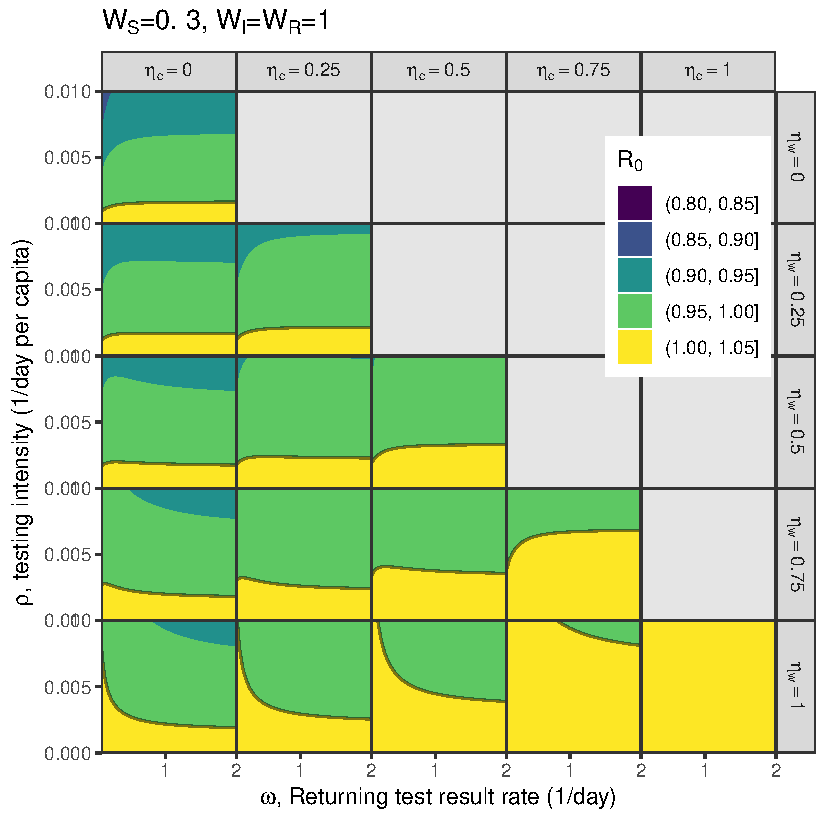
\includegraphics[width=\linewidth]{codes/R0contour_TTI.pdf}
\caption{}\label{p.b}
\end{subfigure}
\caption{
{\bf Effectiveness of testing and isolation in reducing $\Rnum$ at low \percap testing intensity ($\rho$).}
Numerical evaluation of the effectiveness of control ($\Delta$: eq.~\ref{eq:del4a}), over a range of testing and isolation parameters. Parameter values (Table~\ref{tab:params}):
$\beta=\betaparam/$day, $1/\gamma= \invgammaparam$ days (baseline $\Rnum=\Rnumparam$, $r=\rparam$); $\omega \in [1/12,2]/$day;  $\rho \in [0,0.013]/$day per capita; $\theta\_w$ and $\theta\_c$ vary between 0 (no effect of isolation) and 1 (complete elimination of transmission); $p_S=0$, $p_I=1$ and $p_R=0.5$. Only parameter sets where $\theta\_c \geq \theta\_w$ (confirmed-positive individuals isolate more effectively than waiting individuals) are shown; the alternative case, $\theta\_w > \theta\_c$, is unrealistic. Contours of $\Delta$ are plotted for (a) random testing ($w_S=w_I=w_R=1$) and (b) targeted testing ($w_S=0.3$; $w_I=w_R=1$). 
}
\label{pan}
\end{figure}

\begin{figure}[h!]
\centering
\begin{subfigure}[t]{.49\textwidth}
\centering
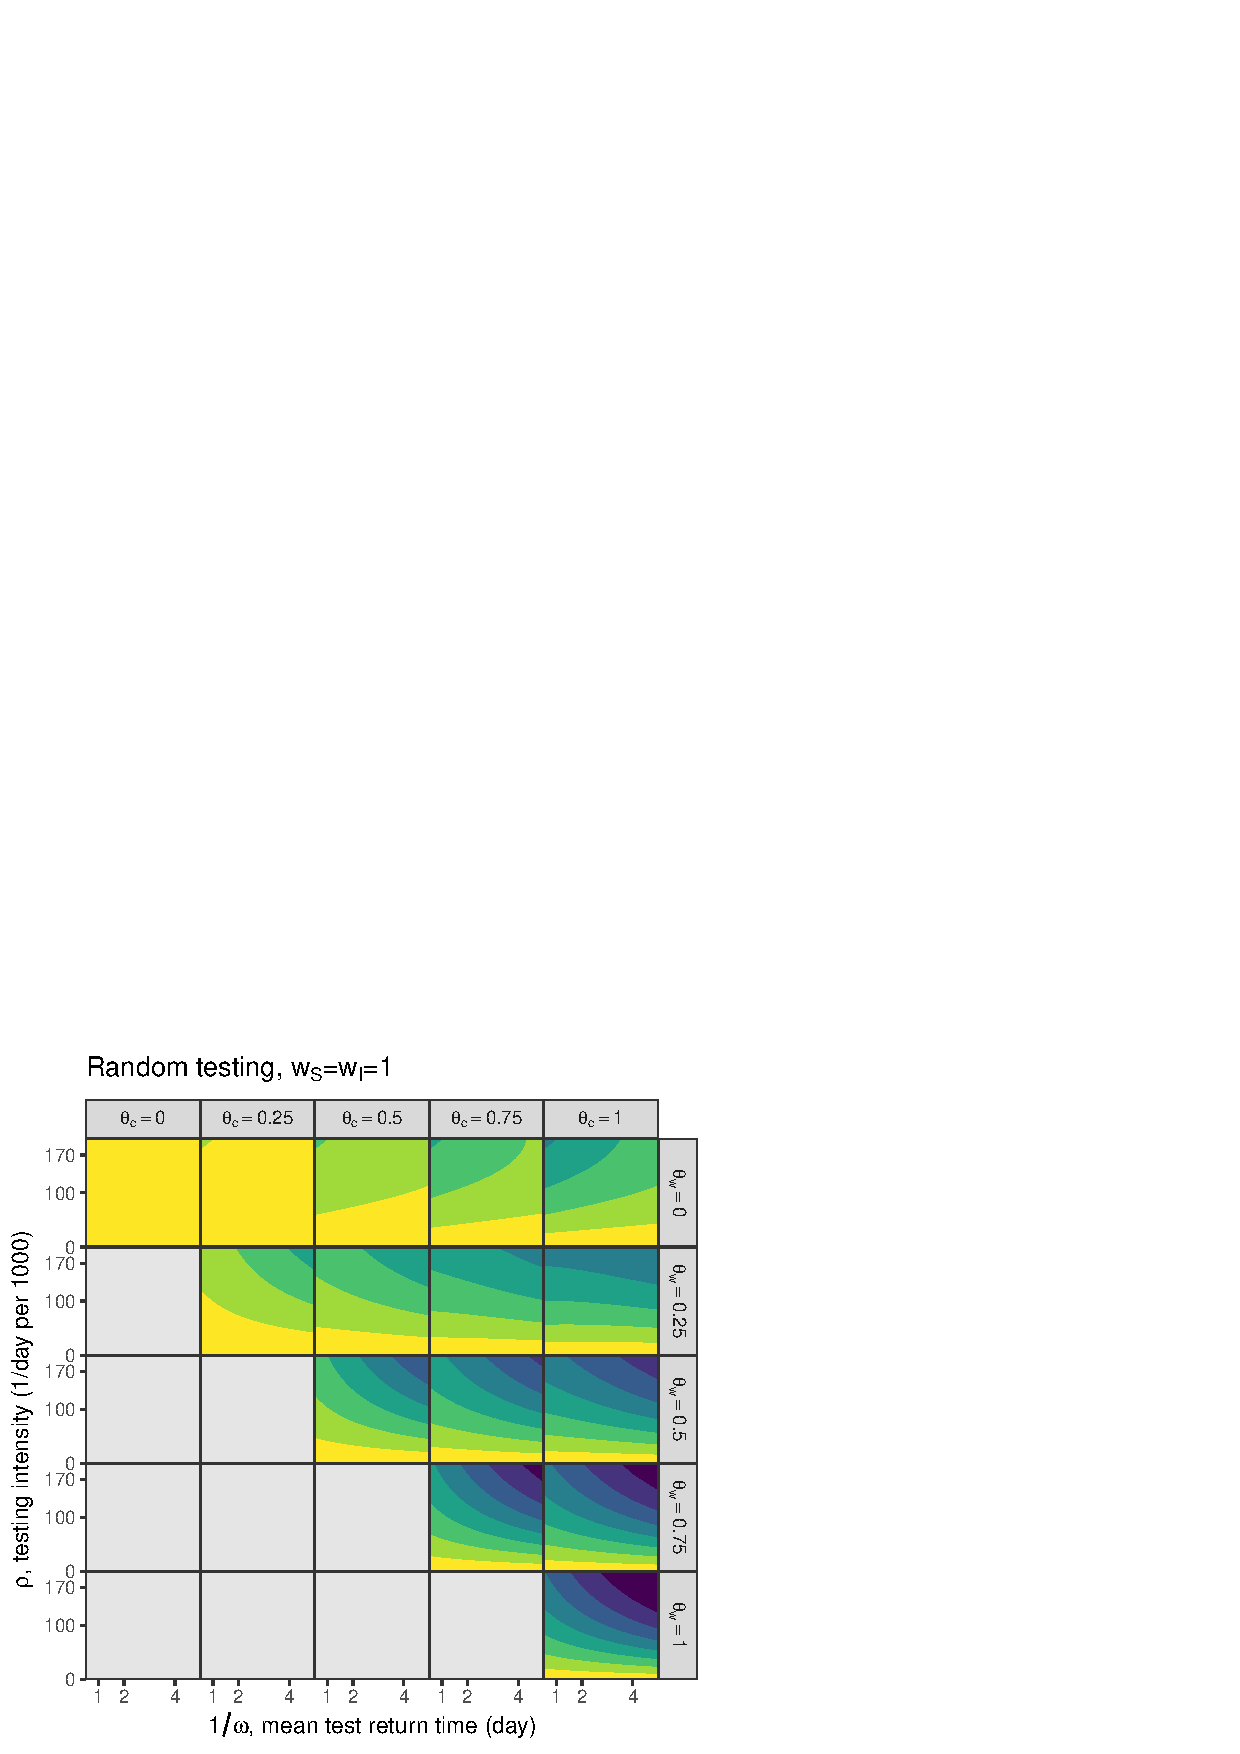
\includegraphics[width=\linewidth]{codes/R0contour_random2.pdf}
\caption{}
\end{subfigure}
%
\begin{subfigure}[t]{.49\textwidth}
\centering
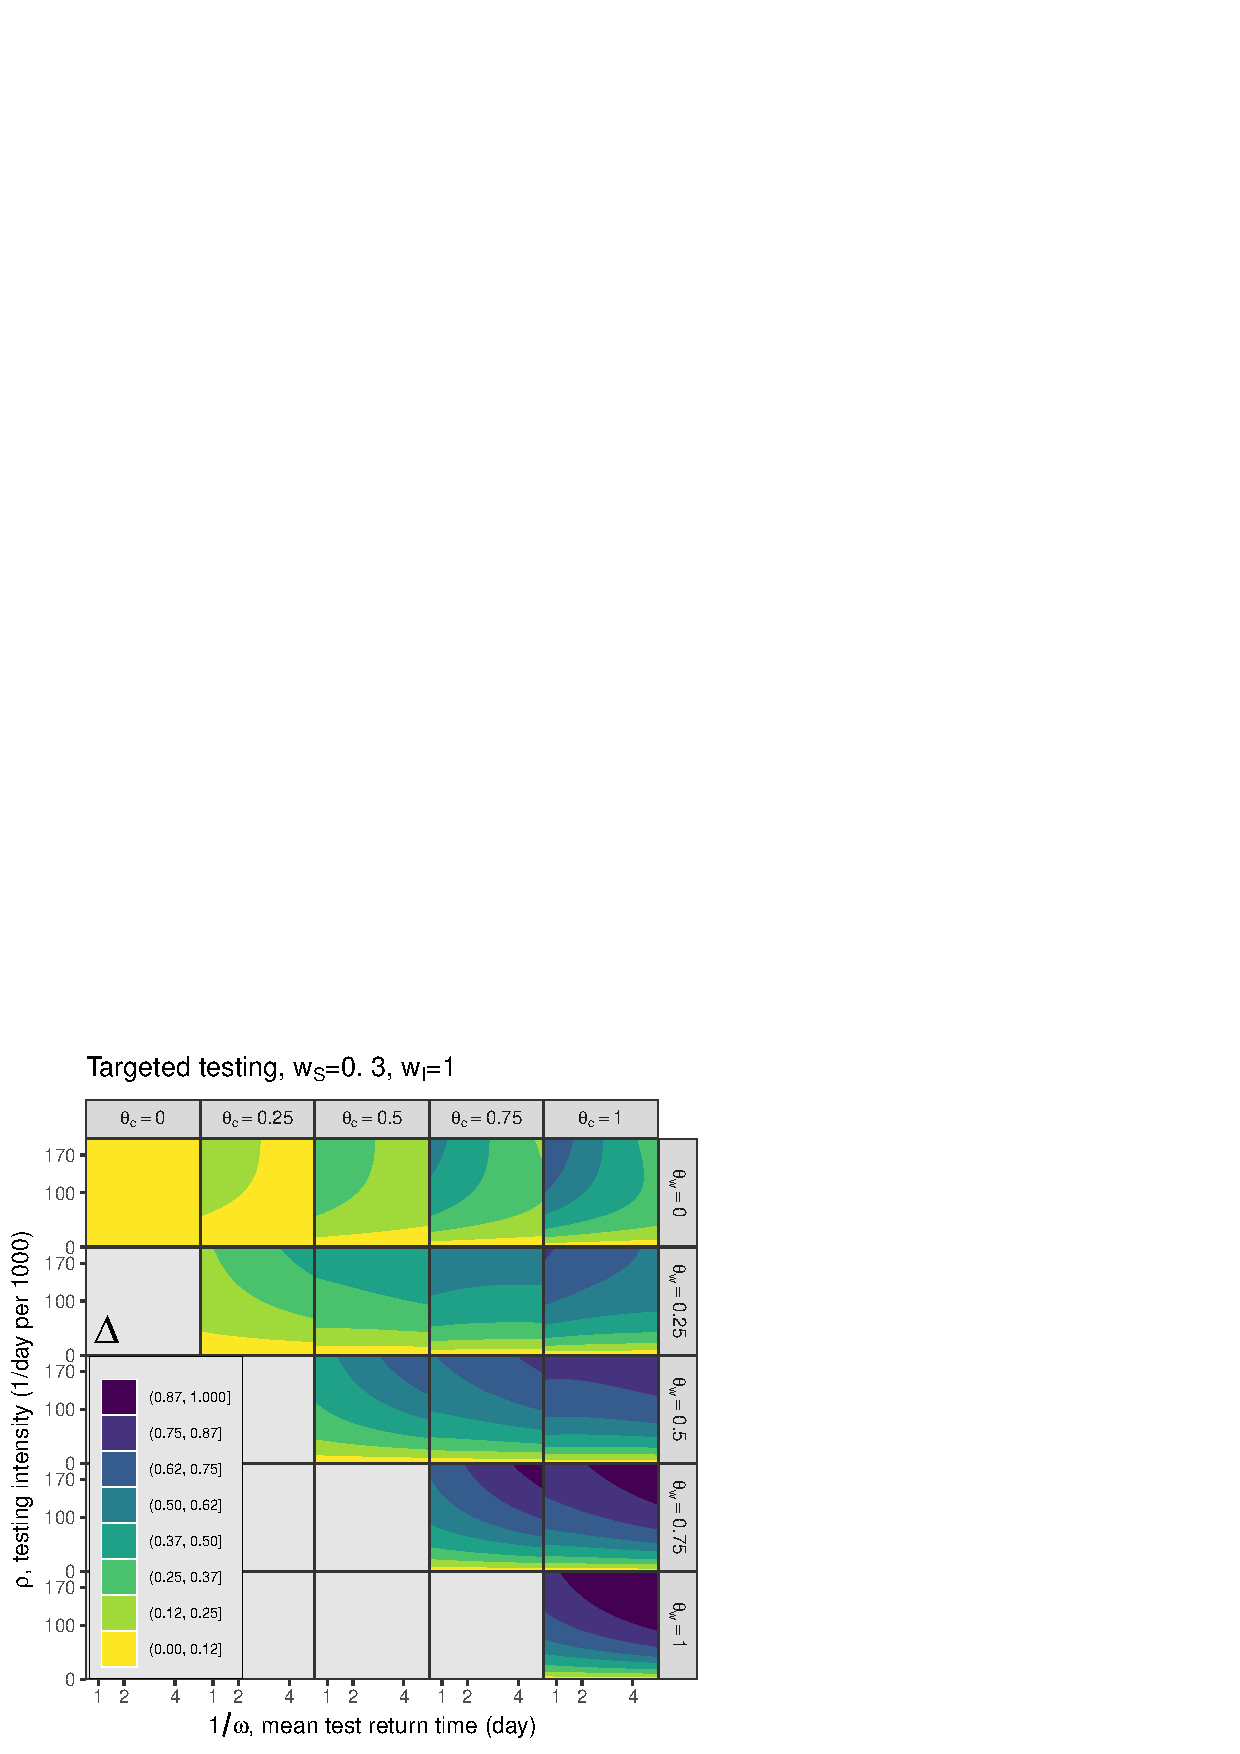
\includegraphics[width=\linewidth]{codes/R0contour_TTI2.pdf}
\caption{}
\end{subfigure}
\caption{
  {\bf Effectiveness of testing and isolation in reducing $\Rnum$ at high \percap testing intensity.}
  Numerical evaluation of the effectiveness of control ($\Delta$: eq.~\ref{eq:del4a}), over a range of testing and isolation parameters. Parameters as in \fref{pan} except: $\omega \in [1/5,2]/$day, $\rho \in [0,1/5)/$day. As in \fref{pan}, subplots show (a) random testing where $w_S=w_I=w_R=1$ and (b) targeted testing where $w_S=0.3$ and $w_I=w_R=1$.
}
\label{pan2}
\end{figure}

However, there are also two specific cases where $\Delta$ changes non-monotonically, in counterintuitive directions, as a function of testing and isolation parameters.

\begin{itemize}
\item We would generally expect increasing testing delays to increase \Rnum, thus decreasing effectiveness of control $\Delta$. This is in fact what happens when waiting individuals do not isolate ($\theta\_w =0$, top row of \fref{pan}) --- as we move to the right within each plot in this row, $\Delta$ decreases.
However, when waiting individuals isolate ($\theta\_w>0$), we more often see the opposite effect: longer testing delays lead to a greater control effect $\Delta$ (reduced $\Rnum$). The reason is that people waiting for negative tests are assumed to continue to isolate; this applies both to susceptibles and to people who became infected while waiting for negative test results. This effect outweighs the effect of confirmed individuals isolating, except when this isolation parameter ($\theta\_c$) is substantially greater than $\theta\_w$. This result depends on the idea that, all else equal, people who have to wait longer for test results isolate at the same level (but for a longer time) as they would if the wait were shorter.
\item \fref{pan} also shows that greater testing intensity (increasing $\rho$) generally increases the effectiveness of control (moving up in each panel). However, this relationship can be reversed at very high testing intensities (provided testing is targeted, and $\theta\_w$ is relatively small; \fref{pan2}(b), right three panels of top row). It is theoretically possible for increasing testing intensity to \emph{increase} \Rnum because more rapid testing leaves more susceptibles in the ``waiting-for-negative-results'' category at the DFE; if these people become infected while waiting, they will need to wait for their negative test result before they can be tested again, receive a positive test, and then begin self-isolating. This effect is usually weak compared to the beneficial effects of testing.

\end{itemize}
